\documentclass[aspectratio=169]{beamer}

\mode<presentation>
{
  \usetheme{default}
  \usecolortheme{default}
  \usefonttheme{default}
  \setbeamertemplate{navigation symbols}{}
  \setbeamertemplate{caption}[numbered]
  \setbeamertemplate{footline}[frame number]  % or "page number"
  \setbeamercolor{frametitle}{fg=white}
  \setbeamercolor{footline}{fg=black}
} 

\usepackage[english]{babel}
\usepackage[utf8x]{inputenc}
\usepackage{tikz}
\usepackage{courier}
\usepackage{array}
\usepackage{bold-extra}
\usepackage{minted}
\usepackage[thicklines]{cancel}
\usepackage{tabularx}

\xdefinecolor{dianablue}{rgb}{0.18,0.24,0.31}
\xdefinecolor{darkblue}{rgb}{0.1,0.1,0.7}
\xdefinecolor{darkgreen}{rgb}{0,0.5,0}
\xdefinecolor{darkgrey}{rgb}{0.35,0.35,0.35}
\xdefinecolor{darkorange}{rgb}{0.8,0.5,0}
\xdefinecolor{darkred}{rgb}{0.7,0,0}
\definecolor{darkgreen}{rgb}{0,0.6,0}
\definecolor{mauve}{rgb}{0.58,0,0.82}

\title[2017-12-08-uproot-update]{\Huge uproot update}
\author{Jim Pivarski}
\institute{Princeton University -- DIANA-HEP}
\date{December 12, 2017}

\begin{document}

\logo{\pgfputat{\pgfxy(0.11, 7.4)}{\pgfbox[right,base]{\tikz{\filldraw[fill=dianablue, draw=none] (0 cm, 0 cm) rectangle (50 cm, 1 cm);}\mbox{\hspace{-8 cm}
\includegraphics[height=1 cm]{princeton-logo-long.png}
\includegraphics[height=1 cm]{diana-hep-logo-long.png}}}}}

\begin{frame}
  \titlepage
\end{frame}

\logo{\pgfputat{\pgfxy(0.11, 7.4)}{\pgfbox[right,base]{\tikz{\filldraw[fill=dianablue, draw=none] (0 cm, 0 cm) rectangle (50 cm, 1 cm);}\mbox{\hspace{-8 cm}
\includegraphics[height=1 cm]{princeton-logo.png}
\includegraphics[height=1 cm]{diana-hep-logo.png}}}}}

% Uncomment these lines for an automatically generated outline.
%\begin{frame}{Outline}
%  \tableofcontents
%\end{frame}

% START START START START START START START START START START START START START

\begin{frame}{(Everybody check out the ZEBRA manual!)}
\vspace{0.6 cm}
\begin{center}
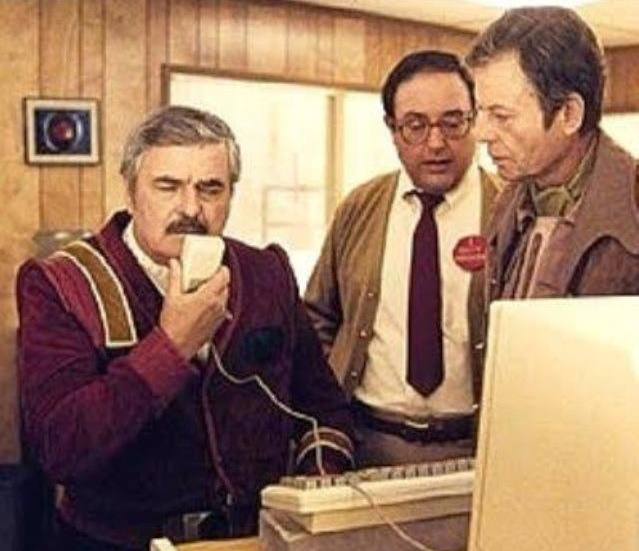
\includegraphics[height=6 cm]{scotty.jpg}

\LARGE ``Hello, computer?''
\end{center}
\end{frame}

\begin{frame}{``Data bank'' management systems}
\vspace{0.25 cm}
\begin{center}
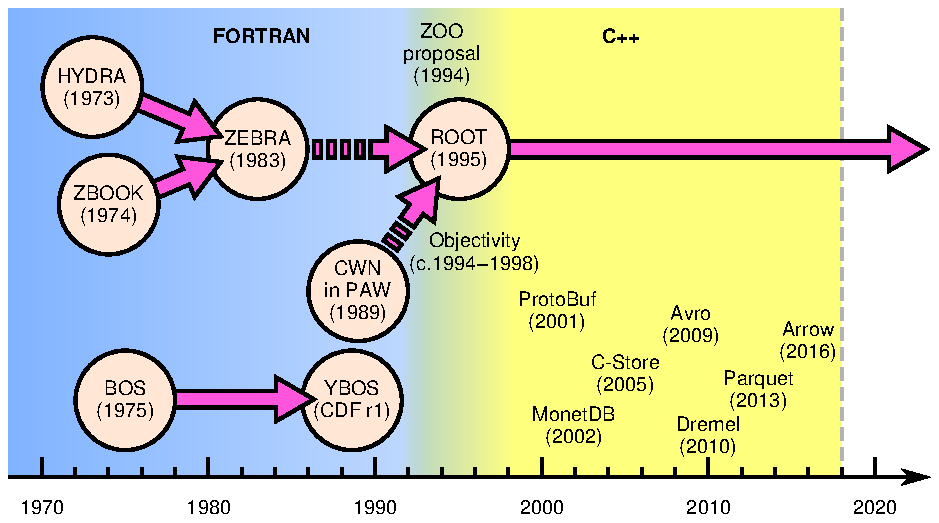
\includegraphics[width=0.95\linewidth]{history.pdf}
\end{center}
\end{frame}

\begin{frame}{File formats {\it and specifications}}
\vspace{0.5 cm}
\begin{columns}
\column{1.1\linewidth}
\renewcommand{\arraystretch}{1.5}
\begin{tabular}{l c c c}
& inception & specification & implementations \\\hline

FITS & 1981 & \href{https://fits.gsfc.nasa.gov/standard30/fits_standard30aa.pdf}{\textcolor{blue}{\tiny https://fits.gsfc.nasa.gov/standard30/fits\_standard30aa.pdf}} & 38 \\

netCDF,HDF4/5 & 1992 & \href{https://support.hdfgroup.org/HDF5/doc/H5.format.html}{\textcolor{blue}{\tiny https://support.hdfgroup.org/HDF5/doc/H5.format.html}} & 35 \\

ROOT & 1995 & {\tiny some class headers like \href{https://root.cern.ch/doc/master/classTFile.html}{\textcolor{blue}{TFile}} and \href{https://root.cern.ch/doc/master/classTKey.html}{\textcolor{blue}{TKey}}; not enough info to read a file} & 6 \\

Pickle & 1996 & {\tiny {\it implementation} changes: 1$\to$2 \href{http://legacy.python.org/dev/peps/pep-0307/}{\textcolor{blue}{PEP-307}}, 3$\to$4 \href{https://www.python.org/dev/peps/pep-3154/}{\textcolor{blue}{PEP-3154}}; not a real spec} & 4 \\

Protocol buffers & 2001 & \href{https://developers.google.com/protocol-buffers/docs/encoding}{\textcolor{blue}{\tiny https://developers.google.com/protocol-buffers/docs/encoding}} & 20 \\

Thrift & 2007 & {\tiny {\bf UNOFFICIAL:} \href{https://erikvanoosten.github.io/thrift-missing-specification/}{\textcolor{blue}{\tiny https://erikvanoosten.github.io/thrift-missing-specification/}}} & 15 \\

Avro & 2009 & \href{http://avro.apache.org/docs/current/spec.html}{\textcolor{blue}{\tiny http://avro.apache.org/docs/current/spec.html}} & 13 \\

Parquet & 2013 & \href{http://parquet.apache.org/documentation/latest/}{\textcolor{blue}{\tiny http://parquet.apache.org/documentation/latest/}} & 5 \\

Arrow/Feather & 2016 & \href{https://arrow.apache.org/docs/memory_layout.html}{\textcolor{blue}{\tiny https://arrow.apache.org/docs/memory\_layout.html}} & 7 \\
\end{tabular}
\end{columns}
\end{frame}

\begin{frame}{Same table, as a plot}
\vspace{0.25 cm}
\begin{columns}
\column{0.7\linewidth}
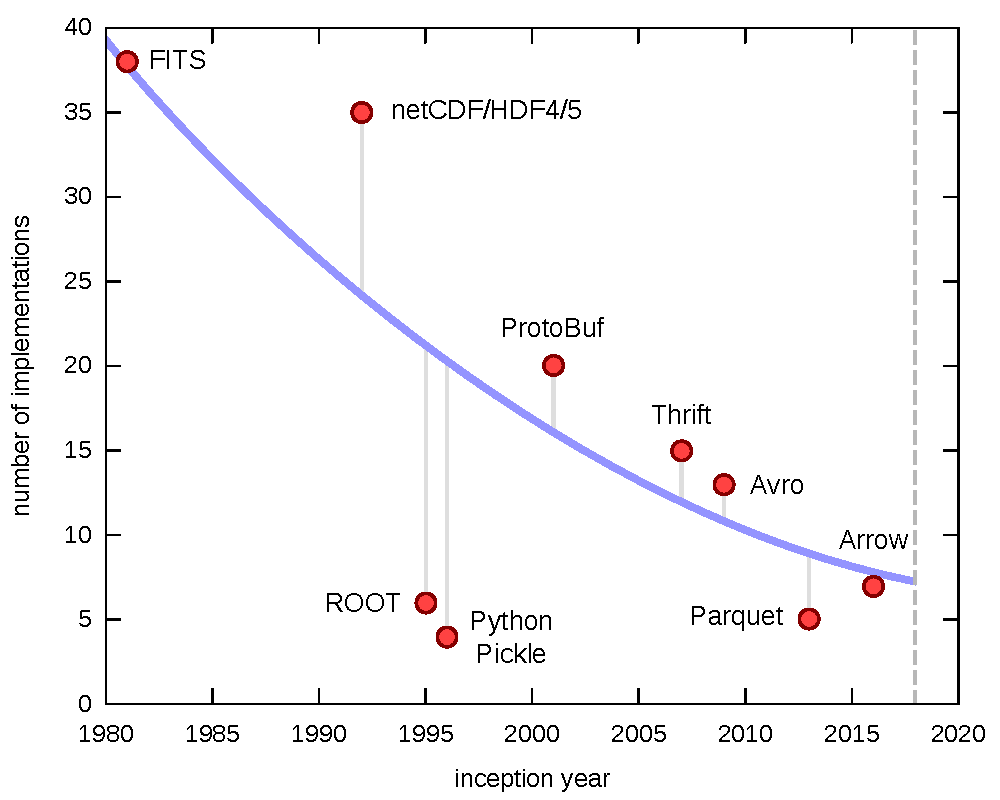
\includegraphics[width=\linewidth]{specs.pdf}

\column{0.35\linewidth}
\textcolor{darkblue}{\underline{General trend}}

\vspace{0.1 cm}
File formats that are used for many years tend to accrete implementations, to access the data in different ways.

\small

\vspace{0.4 cm}
\uncover<2->{\textcolor{darkblue}{Outlier:} netCDF/HDF4/5 may be too broad to call one format.}

\vspace{0.2 cm}
\uncover<3->{\textcolor{darkblue}{Outlier:} Python Pickle is only reimplemented when the whole language is reimplemented.}

\vspace{0.2 cm}
\uncover<4->{\textcolor{darkblue}{Outlier:} the ROOT format is not defined by a specification, making it hard to reimplement.}

\end{columns}
\end{frame}

\begin{frame}{ROOT I/O implementations}
\vspace{0.25 cm}
\begin{columns}
\column{1.1\linewidth}
\renewcommand{\arraystretch}{1.6}
\begin{tabular}{p{2 cm} c p{4.7 cm} p{5.25 cm}}
\centering ROOT & C++ & ROOT itself. & The ROOT Team \\
\centering JsRoot & Javascript & For interacting with ROOT in web browsers or standalone & Bertrand Bellenot, Sergey Linev (within the ROOT Team) \\
\centering root4j/ spark-root & Java/Scala & For Spark and other Big Data projects that run on Java & Started by Tony Johnson in 2001, updated by Viktor Khristenko \\
\centering inlib/exlib & C++ & Intended as an alternative, embedded in GEANT-4 & Guy Barrand \\
\centering rootio & Go & go-hep ecosystem in Go & Sebastien Binet \\
\centering \only<1>{\textcolor{black}{uproot}}\only<2>{\textcolor{blue}{uproot}} & \only<1>{\textcolor{black}{Python}}\only<2>{\textcolor{blue}{Python}} & \only<1>{\textcolor{black}{For quickly getting ROOT data into Numpy and Pandas for machine learning}}\only<2>{\textcolor{blue}{For quickly getting ROOT data into Numpy and Pandas for machine learning}} & \only<1>{\textcolor{black}{Jim Pivarski (me)}}\only<2>{\textcolor{blue}{Jim Pivarski (me)}} \\
& \textcolor{gray}{Rust?} & \textcolor{gray}{(typesafe object ownership} & \mbox{\hspace{-0.7 cm}\textcolor{gray}{without a garbage collector)}} \\
\end{tabular}
\end{columns}
\end{frame}

\begin{frame}{Motivations for uproot}
\vspace{0.25 cm}
\begin{center}
\only<1>{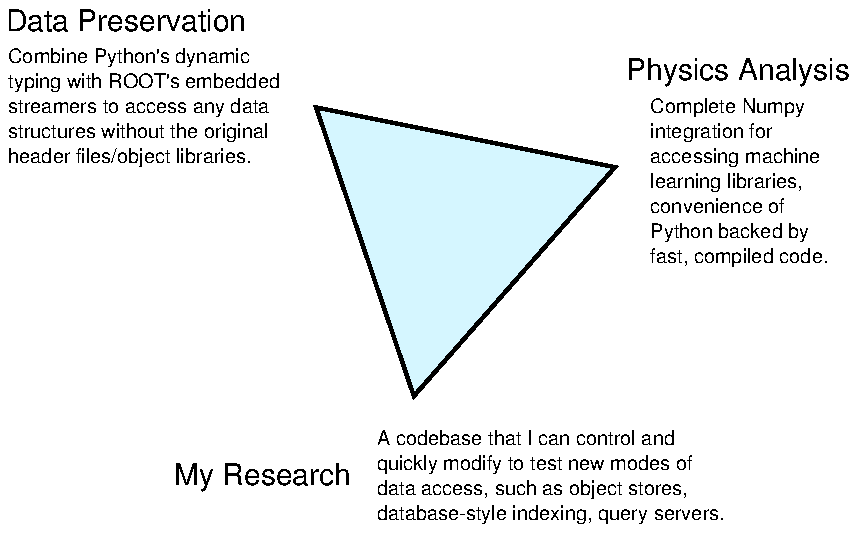
\includegraphics[width=0.85\linewidth]{motivations.pdf}}
\only<2>{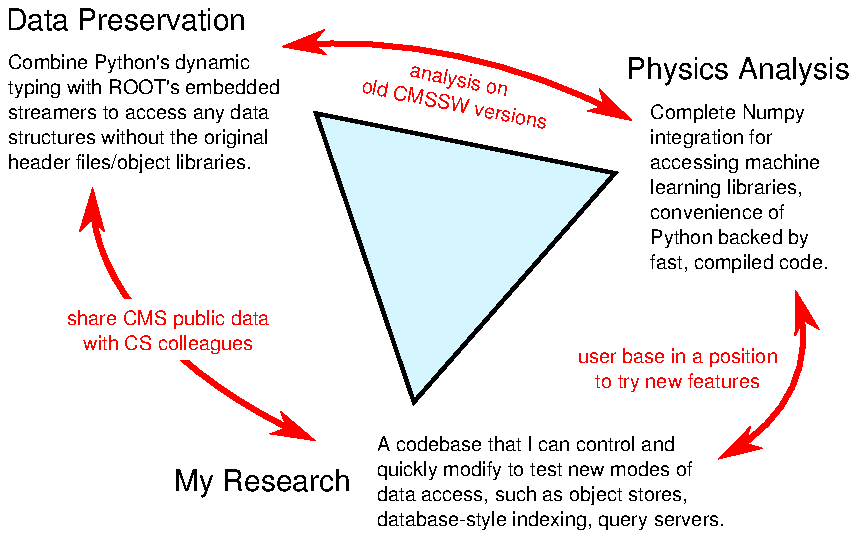
\includegraphics[width=0.85\linewidth]{motivations-2.pdf}}
\end{center}
\end{frame}

\begin{frame}{Let's try something dangerous}
\vspace{0.5 cm}
\Large
\begin{itemize}\setlength{\itemsep}{0.3 cm}
\item The safest thing I could do is keep showing high-level slides, without getting into the code itself.
\item<2-> It would be more dangerous to attempt a live demo. No matter how well you prepare, the Demo Gods will smite you.
\item<3-> Worse still, I'm going to ask you to download it and apply it to your own data while I show examples of what {\it should} work.
\end{itemize}

\large
\vspace{0.5 cm}
\uncover<4->{You will find bugs. Not all of them will be real. Ask me or a neighbor to take a look at it; if the problem isn't obvious, submit a bug report with a small test file. Thanks!}
\end{frame}

\begin{frame}[fragile]{Here it goes\ldots}
\vspace{0.5 cm}
\huge
\begin{center}
\begin{minipage}{0.8\linewidth}
\begin{verbatim}
pip install uproot --user
\end{verbatim}
\end{minipage}

\Large
\begin{uncoverenv}<2->
\vspace{1 cm}
\href{https://github.com/scikit-hep/uproot}{\textcolor{blue}{https://github.com/scikit-hep/uproot}}

\vspace{0.5 cm}
\href{http://uproot.readthedocs.io}{\textcolor{blue}{http://uproot.readthedocs.io}}

\vspace{0.5 cm}
\href{https://groups.google.com/forum/#!forum/uproot-users/join}{\textcolor{blue}{https://groups.google.com/forum/\#!forum/uproot-users/join}}
\end{uncoverenv}
\end{center}
\end{frame}

\begin{frame}{Roadmap and scope}
\vspace{0.5 cm}
\large
\begin{description}\setlength{\itemsep}{0.5 cm}
\item[version 1.x] \textcolor{darkblue}{\it (last talk here)} minimalistic ROOT-to-Numpy implementation because this feature was delayed in ROOT 6.12.

\item[version 2.x] \textcolor{darkblue}{\it (current)} a complete rewrite using ROOT streamers to recognize any data type. Anything can now be read from TDirectories but currently only numbers, strings, and {\tt std::vector<number>} can be read from TTrees.

\vspace{0.5 cm}
Classes that have been ``split'' (the default) usually satisfy the above.

\item[version 3.x] \textcolor{darkblue}{\it (future)} will add the ability to write files. Will be limited to reading from one file and writing to another.
\end{description}
\end{frame}

\begin{frame}{Terminology (may refer back to this slide)}
\vspace{0.25 cm}
\begin{center}
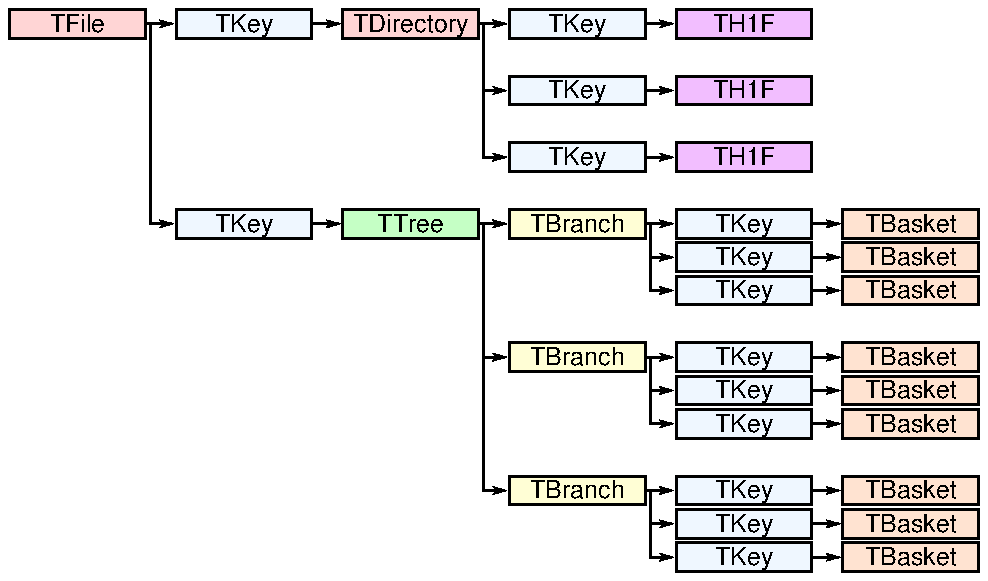
\includegraphics[width=0.9\linewidth]{terminology.pdf}
\end{center}
\end{frame}

\begin{frame}{Levels of trustworthiness}
\vspace{-0.1 cm}
\large
\renewcommand{\arraystretch}{4}
\begin{tabular}{p{2 cm} p{10 cm}}
\parbox[c]{1.5 cm}{
\includegraphics[width=1.5 cm]{safe.png}} & The feature in question is an essential part of the codebase; I designed around it and have included a formal test suite. Also, there's documentation (references, docstrings). \\
\parbox[c]{1.5 cm}{
\includegraphics[width=1.5 cm]{caution.png}} & Mostly the same code paths as above and {\it informally} tested, but not yet integrated into the formal tests. \\
\parbox[c]{1.5 cm}{
\includegraphics[width=1.5 cm]{danger.png}} & I wrote the feature for this talk and have only tested the examples shown here. \\
\end{tabular}
\end{frame}

\begin{frame}[fragile]{The basics: poking around}
\vspace{0.1 cm}
\small
\begin{minted}{python}
>>> import uproot
>>> f = uproot.open("~/TrackResonanceNtuple.root")
>>> f.keys()
\end{minted}
\begin{verbatim}
['TrackResonanceNtuple;1']
\end{verbatim}
\begin{minted}{python}
>>> f.allkeys()
\end{minted}
\begin{verbatim}
['TrackResonanceNtuple;1', 'TrackResonanceNtuple/twoTrack;2',
 'TrackResonanceNtuple/twoTrack;1',
 'TrackResonanceNtuple/twoMuon;1']
\end{verbatim}
\begin{minted}{python}
>>> f.classes()
\end{minted}
\begin{verbatim}
[('TrackResonanceNtuple;1', <class 'uproot.rootio.ROOTDirectory'>)]
\end{verbatim}
\begin{minted}{python}
>>> f["TrackResonanceNtuple"].classes()
\end{minted}
\begin{verbatim}
[('twoTrack;2', <class 'uproot.rootio.TTree'>),
 ('twoTrack;1', <class 'uproot.rootio.TTree'>),
 ('twoMuon;1', <class 'uproot.rootio.TTree'>)]
\end{verbatim}

\vspace{-7.6 cm}
\hfill 
\includegraphics[width=1.5 cm]{safe.png}\hspace{-0.9 cm}
\vspace{7.5 cm}
\end{frame}

\begin{frame}[fragile]{The basics: getting data from a TTree}
\vspace{0.1 cm}
\small
\begin{minted}{python}
>>> import uproot
>>> t = uproot.open("tests/samples/Zmumu.root")["events"]
>>> t.keys()
\end{minted}
\begin{verbatim}
['Type', 'Run', 'Event', 'E1', 'px1', 'py1', 'pz1', 'pt1',
 'eta1', 'phi1', 'Q1', 'E2', 'px2', 'py2', 'pz2', 'pt2',
 'eta2', 'phi2', 'Q2', 'M']
\end{verbatim}
\begin{minted}{python}
>>> t["M"].array()
\end{minted}
\begin{verbatim}
array([ 82.46269156,  83.62620401,  83.30846467, ...,  95.96547966,
        96.49594381,  96.65672765])
\end{verbatim}
\begin{minted}{python}
>>> t.arrays(["px1", "py1", "pz1"])
\end{minted}
\begin{verbatim}
{'py1': array([ 17.433243, -16.5703623, -16.5703623, ..., 1.1994057,
 ...
\end{verbatim}
\begin{minted}{python}
>>> t.arrays()    # all of them!
\end{minted}
\begin{verbatim}
 ...
\end{verbatim}
\vspace{-7.6 cm}
\hfill 
\includegraphics[width=1.5 cm]{safe.png}\hspace{-0.9 cm}
\vspace{7.5 cm}
\end{frame}

\begin{frame}[fragile]{The basics: doing meaningful calculations with them}
\vspace{0.5 cm}
\small
\begin{minted}{python}
>>> import numpy
>>> for px,py,pz in t.iterate(["px1","py1","pz1"], outputtype=tuple):
...     pt = numpy.sqrt(px**2 + py**2)
...     eta = numpy.arctanh(pz / numpy.sqrt(px**2 + py**2 + pz**2))
...     phi = numpy.arctan2(py, px)
...     print(pt)
...     print(eta)
...     print(phi)
... 
\end{minted}
\begin{verbatim}
[ 44.7322 38.8311  38.8311  ...,  32.3997  32.3997 32.5076  ]
[-1.21769 -1.05139 -1.05139 ..., -1.57044 -1.57044 -1.57078 ]
[ 2.74126 -0.44087 -0.44087 ...,  0.03702  0.03702  0.036964]
\end{verbatim}

\vspace{0.5 cm}
Also {\tt uproot.iterate("$\sim$/files*.root", "events", ...)} for a collection of files.

\vspace{-4.5 cm}
\hfill 
\includegraphics[width=1.5 cm]{safe.png}\hspace{-0.9 cm}
\vspace{4.5 cm}
\end{frame}

\begin{frame}[fragile]{Connector to an external package: Pandas}
\vspace{0.25 cm}
\small
\begin{minted}{bash}
$ pip install pandas --user
\end{minted}
\begin{minted}{python}
>>> df = t.pandas.df()   # all the same arguments as t.arrays()
>>> df
\end{minted}
\begin{verbatim}
              E1          E2      Event          M  Q1  Q2     Run  \
0      82.201866   60.621875   10507008  82.462692   1  -1  148031
1      62.344929   82.201866   10507008  83.626204  -1   1  148031
2      62.344929   81.582778   10507008  83.308465  -1   1  148031
3      60.621875   81.582778   10507008  82.149373  -1   1  148031
...
2302   1.199406 -26.398400  -74.532431 -153.847604   GT
2303   1.201350 -26.398400  -74.808372 -153.847604   GG

[2304 rows x 20 columns]
\end{verbatim}

\vspace{0.25 cm}
Then search the web to learn how to do exploratory analysis, make plots, apply machine learning algorithms, etc. (Or read the {\it Python for Data Analysis} book.)

\vspace{-3 cm}
\hfill 
\includegraphics[width=1.5 cm]{caution.png}\hspace{-0.9 cm}
\vspace{3 cm}
\end{frame}

\begin{frame}[fragile]{Accessing data of non-uniform width (not scalar numbers)}
\vspace{0.25 cm}
\small
\begin{minted}{python}
>>> t = uproot.open("tests/samples/mc10events.root")["Events"]
>>> a = t.array("Muon.pt")    # such as std::vector<numbers>
>>> a                         # variable length for each event
\end{minted}
\begin{verbatim}
jaggedarray([[ 28.07074928],
             [],
             [ 5.52336693  5.4780116 4.13222885],
             ...
             [],
             [ 6.85138178],
             []])
\end{verbatim}
\begin{uncoverenv}<2->
\begin{minted}{python}
>>> a.contents
\end{minted}
\begin{verbatim}
array([ 28.07074928,   5.52336693,   5.47801161,   4.13222885, ...
         5.06344414,   6.85138178], dtype=float32)
\end{verbatim}
\begin{minted}{python}
>>> a.stops
\end{minted}
\begin{verbatim}
array([ 1,  1,  4,  7,  7,  8, 13, 13, 14, 14])
\end{verbatim}
\end{uncoverenv}

\vspace{-7.7 cm}
\hfill 
\includegraphics[width=1.5 cm]{safe.png}\hspace{-0.9 cm}
\vspace{7.7 cm}
\end{frame}

\begin{frame}[fragile]{Also, strings! (can store any variable-width data in jagged array)}
\vspace{0.5 cm}
\small
\begin{minted}{python}
>>> a = uproot.open("foriter2.root")["foriter2"]["data"]
>>> a
\end{minted}
\begin{verbatim}
strings(['zero' 'one' 'two' ... 'twenty-nine' 'thirty'])
\end{verbatim}
\begin{uncoverenv}<2->
\begin{minted}{python}
>>> a.jaggedarray.contents
\end{minted}
\begin{verbatim}
array([122, 101, 114, 111, 111, 110, 101, 116, 119, 111, 116, 104,
       114, 101, 101, 102, 111, 117, 114, 102, 105, 118, 101, 115,
       ...
       101, 105, 103, 104, 116, 116, 119, 101, 110, 116, 121,  45,
       110, 105, 110, 101, 116, 104, 105, 114, 116, 121], dtype=uint8)
\end{verbatim}
\begin{minted}{python}
>>> a.jaggedarray.stops
\end{minted}
\begin{verbatim}
array([  4,   7,  10,  15,  19,  23,  26,  31,  36,  40,  43,  49,
       ...
       179, 191, 203, 214, 220])
\end{verbatim}
\end{uncoverenv}
\vspace{-7 cm}
\hfill 
\includegraphics[width=1.5 cm]{safe.png}\hspace{-0.9 cm}
\vspace{7 cm}
\end{frame}

\begin{frame}[fragile]{As complex as STL vectors in a MiniAOD file}
\vspace{0.25 cm}
\small
\begin{minted}{python}
>>> t = uproot.open("~/cmssw-miniaod.root")["Events"]
\end{minted}
\begin{verbatim}
>>> for basket in (t["GenEventInfoProduct_generator__HLT.obj.weights_"]
                   .iterate_baskets()):
...     print(basket)
...
[[  1.000000e+00   4.201630e-05 ...   4.242230e-05   3.990430e-05],
 [  1.000000e+00   4.201630e-05 ...   2.648060e-05   2.773620e-05],
 [  1.000000e+00   4.201630e-05 ...   4.329220e-05   4.058060e-05],
 ...
\end{verbatim}

\vspace{0.25 cm}
{\normalsize Though uproot was designed for analysis-ready TTrees, it will someday cover all data types by using the streamer info provided in each file.}

\vspace{-0.2 cm}
\hfill 
\includegraphics[width=1.5 cm]{caution.png}\hspace{-0.9 cm}
\end{frame}

\begin{frame}[fragile]{Can already read arbitrary objects from TDirectory}
\vspace{0.25 cm}
\small
\begin{minted}{python}
>>> f = uproot.open("~/histograms.root")
>>> f.allclasses()
\end{minted}
\begin{verbatim}
[('one;1', <class 'uproot.rootio.TH1F'>), ('two;1', <class 'uproot.rootio.TH1F'>),
 ('three;1', <class 'uproot.rootio.TH1F'>)]
\end{verbatim}
\begin{minted}{python}
>>> hist = f["one"]
>>> for n, v in hist.__dict__.items():   # class generated on the fly
...     if n.startswith("f"):            # with all the private fields
...         print n + "\t", v
...
\end{minted}
\begin{verbatim}
fMarkerStyle    1
fMaximum        -1111.0
fEntries        10000.0
fLineColor      602
fContour        []
fYaxis  <TAxis 'yaxis' at 0x7e3a12cfee50>
fTsumwx2        10388.1526213
\end{verbatim}

\vspace{-7.7 cm}
\hfill 
\includegraphics[width=1.5 cm]{safe.png}\hspace{-0.9 cm}
\vspace{7.7 cm}
\end{frame}

\begin{frame}[fragile]{Some classes are endowed with Python methods}
\vspace{0.5 cm}
Histogram inspection and manipulation:
\small
\begin{minted}{python}
>>> hist.numbins, hist.low, hist.high
\end{minted}
\begin{verbatim}
(10, -3.0, 3.0)
\end{verbatim}
\begin{minted}{python}
>>> hist.values
\end{minted}
\begin{verbatim}
[68.0, 285.0, 755.0, 1580.0, 2296.0, 2286.0, 1570.0, 795.0, 289.0, 76.0])
\end{verbatim}
\begin{minted}{python}
>>> hist[4] = 0
>>> hist.values
\end{minted}
\begin{verbatim}
[68.0, 285.0, 755.0, 0, 2296.0, 2286.0, 1570.0, 795.0, 289.0, 76.0]
\end{verbatim}
\begin{minted}{python}
>>> hist.allvalues
\end{minted}
\begin{verbatim}
[0.0, 68.0, 285.0, 755.0, 0, 2296.0, 2286.0, 1570.0, 795.0, 289.0, 76.0, 0.0]
\end{verbatim}
\begin{minted}{python}
>>> hist.underflows, hist.overflows
\end{minted}
\begin{verbatim}
(0.0, 0.0)
\end{verbatim}

\vspace{-7 cm}
\hfill 
\includegraphics[width=1.5 cm]{safe.png}\hspace{-0.9 cm}
\vspace{7 cm}
\end{frame}

\begin{frame}[fragile]{You can always view histograms with a line printer}
\vspace{0.1 cm}
\small
\begin{minted}{python}
>>> hist.show(width=70)
\end{minted}
\begin{verbatim}
                  0                                               2411
                  +--------------------------------------------------+
[-inf, -3)   0    |                                                  |
[-3, -2.4)   68   |*                                                 |
[-2.4, -1.8) 285  |******                                            |
[-1.8, -1.2) 755  |****************                                  |
[-1.2, -0.6) 0    |                                                  |
[-0.6, 0)    2296 |************************************************  |
[0, 0.6)     2286 |***********************************************   |
[0.6, 1.2)   1570 |*********************************                 |
[1.2, 1.8)   795  |****************                                  |
[1.8, 2.4)   289  |******                                            |
[2.4, 3)     76   |**                                                |
[3, inf]     0    |                                                  |
                  +--------------------------------------------------+
\end{verbatim}
\end{frame}

\begin{frame}[fragile]{But you can also use Bokeh as your TCanvas (even remotely)}
\vspace{0.25 cm}
\small
\begin{minted}{bash}
$ pip install bokeh --user
\end{minted}
\begin{minted}{python}
>>> canvas = uproot.BokehCanvas()   # canvas is a singleton
>>> canvas.show()                   # could set hosts="*", port=12345
\end{minted}
\begin{verbatim}
Created new window in existing browser session.
WARNING:tornado.access:404 GET /favicon.ico (::1) 1.09ms
\end{verbatim}
\begin{minted}{python}
>>> hist.bokeh.plot()
>>> uproot.BokehCanvas().url
\end{minted}
\begin{verbatim}
'http://localhost:41712'
\end{verbatim}

\vspace{0.2 cm}
If Python is running on a remote machine, set \\
{\tt hosts="*"} or your IP address (for more security) \\
and manually enter the URL in your web browser.

\vspace{0.2 cm}
The (single) web browser will have a live view of \\
anything you {\tt hist.bokeh.plot()}.

\vspace{-4.25 cm}
\hfill 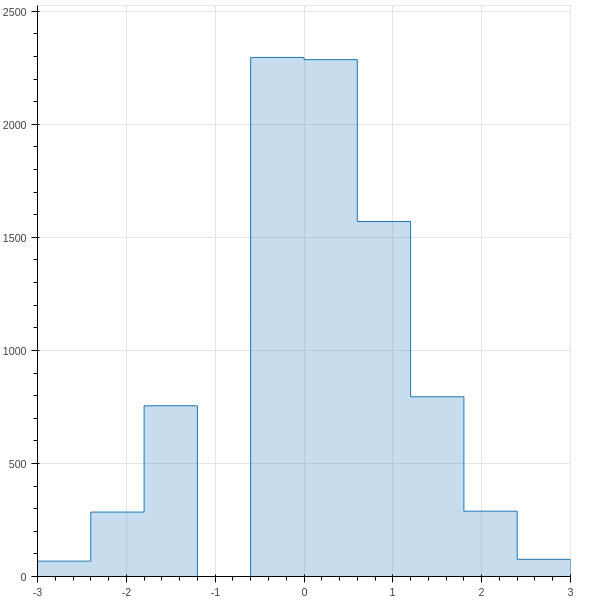
\includegraphics[height=4.5 cm]{bokeh_plot.png}\hspace{1 cm}

\vspace{-2.1 cm}
\hfill 
\includegraphics[width=1.5 cm]{danger.png}\hspace{-0.9 cm}
\vspace{3 cm}
\end{frame}

\begin{frame}[fragile]{Caching intermediate results}
\vspace{0.3 cm}
uproot adheres to the Python philosophy of avoiding implicit actions.

\vspace{0.2 cm}
Caching must be explicit: every time you call {\tt tree.arrays()}, it reads from the file {\it unless a cache is provided.}

\small
\vspace{0.2 cm}
\begin{minted}{python}
>>> t = uproot.open("~/bigfile.root")["Events"]
>>> cache = {}
>>> t.array("Muon.pt", cache=cache)
\end{minted}
\begin{verbatim}
jaggedarray([[ 28.07074928],
             ...,
             [ 33.39884186  30.11572647  14.1813221 ]])
\end{verbatim}
\begin{minted}{python}
>>> cache
\end{minted}
\begin{verbatim}
{'/home/pivarski/bigfile.root;Events;Muon.pt;asjagged(asdtype(Bf4,Lf4,
(),()));0-47407': jaggedarray([[ 28.07074928],
             ...,
             [ 33.39884186  30.11572647  14.1813221 ]])}
\end{verbatim}

\vspace{-6 cm}
\hfill 
\includegraphics[width=1.5 cm]{safe.png}\hspace{-0.9 cm}
\vspace{6 cm}
\end{frame}

\begin{frame}{Caching options}
\vspace{0.25 cm}
Any dict-like object can be a cache. (On the previous page, we used a dict.)

\vspace{0.25 cm}
But dicts don't release objects when running low on memory. Therefore, uproot provides a suite of dict-like objects that {\it do} release the least-recently used (LRU) objects.

\vspace{0.25 cm}
\begin{itemize}
\item {\tt\small uproot.cache.MemoryCache}: a subclass of dict with LRU policy.
\item {\tt\small uproot.cache.ThreadSafeMemoryCache}: same with a lock for multithreading.
\item {\tt\small uproot.cache.DiskCache}: directory of files, uses POSIX operations like linking and file-locking for multi-process safety. Can be resumed after processes exit.
\end{itemize}

\begin{uncoverenv}<2->
\vspace{0.25 cm}
They can be used in any of three arguments:

\vspace{0.25 cm}
\begin{itemize}
\item \textcolor{darkblue}{\it cache:} caches final, fully interpreted arrays.
\item \textcolor{darkblue}{\it basketcache:} caches decompressed TBasket data, to avoid cache-misses when slicing or interpreting the same branch different ways.
\item \textcolor{darkblue}{\it keycache:} tiny TKey data; probably put this in an ordinary dict without LRU.
\end{itemize}
\end{uncoverenv}

\vspace{-7.7 cm}
\hfill 
\includegraphics[width=1.5 cm]{safe.png}\hspace{-0.9 cm}
\vspace{7.7 cm}
\end{frame}

\begin{frame}[fragile]{Similarly, parallel-processing is not implicit}
\vspace{1 cm}
The {\tt\small concurrent.futures} module is part of Python 3 and a package in Python 2.

\small
\begin{minted}{python}
>>> from concurrent.futures import ThreadPoolExecutor
>>> executor = ThreadPoolExecutor(16)
>>> 
>>> t.arrays(["Muon.pt", "Muon.eta", "Muon.phi"], executor=executor)
\end{minted}

\normalsize
\vspace{0.25 cm}
In the above, as many as 16 threads will share the work of
\begin{itemize}
\item reading from disk (memory-mapped file can be multithreaded)
\item decompressing TBaskets belonging to the same TBranch
\item constructing arrays belonging to different TBranches.
\end{itemize}

\vspace{0.25 cm}
Even though Python has a global interpreter lock (GIL), most of the numerical processing is performed in compiled code with the GIL released.

\vspace{-3 cm}
\hfill 
\includegraphics[width=1.5 cm]{safe.png}\hspace{-0.9 cm}
\vspace{3 cm}
\end{frame}

\begin{frame}[fragile]{Non-blocking calls}
\vspace{0.5 cm}
\small
\begin{minted}{python}
>>> results = t.arrays(executor=executor, blocking=False)
>>> results
\end{minted}
\begin{verbatim}
<function await at 0x747a5d2907d0>
\end{verbatim}

\vspace{0.25 cm}
{\normalsize Returns ``await'' function as soon as the work has been {\it submitted} to the executor.}

\vspace{0.25 cm}
{\normalsize To get the result (waiting as long as necessary), call the function:}
\begin{minted}{python}
>>> results()
\end{minted}
\begin{verbatim}
{'CA8Puppi.nNeutrals': jaggedarray([[], [], [], ...,
                                    [], [19 68 14], [10]]),
 'AK4Puppi.hadronFlavor': jaggedarray([[5 0 5 0],
                                       [4 0 5 4 5 0],
                                       [5 0 4 0 0 5],
                                       ...,
\end{verbatim}

\vspace{-2 cm}
\hfill 
\includegraphics[width=1.5 cm]{caution.png}\hspace{-0.9 cm}
\vspace{2 cm}
\end{frame}

\begin{frame}[fragile]{Lazy arrays}
\vspace{0.1 cm}
\small
\begin{minted}{python}
>>> lazy = t.lazyarrays()
>>> lazy
\end{minted}
\begin{verbatim}
{'CA8Puppi.nNeutrals':
     <uproot.tree._LazyArray object at 0x747a5d4f97d0>,
 'AK4Puppi.hadronFlavor':
     <uproot.tree._LazyArray object at 0x747a5d50ff10>,
 ...
\end{verbatim}

\vspace{0.25 cm}
{\normalsize Returns immediately and {\it does no work at all} until/unless you ask for items.}

\vspace{0.25 cm}
\begin{minted}{python}
>>> lazy["Muon.pt"][:100]
\end{minted}
\begin{verbatim}
jaggedarray([[ 28.07074928], ...
\end{verbatim}

\vspace{0.25 cm}
{\normalsize Hint: use with caching to avoid re-reading when asking for the same items twice. Nothing is implicit!}
\begin{minted}{python}
>>> read_only_once = t.lazyarrays(basketcache={})
\end{minted}

\vspace{-7.7 cm}
\hfill 
\includegraphics[width=1.5 cm]{caution.png}\hspace{-0.9 cm}
\vspace{7.7 cm}
\end{frame}

\begin{frame}[fragile]{Numba integration}
\vspace{0.25 cm}
\small
Numba is a just-in-time (JIT) compiler for Python. Install Numba standalone or use CMSSW.

\begin{minted}{bash}
$ conda install numba   # conda, rather than pip, to get LLVM
\end{minted}

\vspace{0.25 cm}
Now any function preceded by {\tt @numba.njit} gets natively compiled \href{http://numba.pydata.org/numba-doc/dev/reference/pysupported.html}{\textcolor{blue}{if Numba knows how}}.

Data structures produced by uproot are Numba-aware.

\begin{minted}{python}
>>> import numba
>>> @numba.njit
... def fillhist(pthist, ptarray):
...     for event in ptarray:
...         for pt in event:
...             pthist.fill(pt)
...     return pthist                   # have to return it
... 
>>> pthist = uproot.hist(100, 0, 50  )  # create empty TH1
>>> ptarray = t.array("Muon.pt")        # jagged array of arrays
>>> pthist = fillhist(pthist, ptarray)  # runs at the speed of C code
>>> pthist.show(width=70)
\end{minted}

\vspace{-5 cm}
\hfill 
\includegraphics[width=1.5 cm]{caution.png}\hspace{-0.9 cm}
\vspace{5 cm}
\end{frame}

\begin{frame}[fragile]{Functional programming}
\vspace{0.25 cm}
\scriptsize
\begin{minted}{python}
>>> t = uproot.open("tests/samples/Zmumu.root")["events"]
>>> from math import sqrt
>>> def mass(E1, px1, py1, pz1, E2, px2, py2, pz2):
...     return sqrt((E1 + E2)**2 - (px1 + px2)**2 - (py1 + py2)**2 - (pz1 + pz2)**2)
... 
>>> t.hist(10, 70, 110, mass).show()
>>> t.filter("E1 > 10 and E2 > 10").hist(10, 70, 110, mass).show()
\end{minted}
\begin{verbatim}
               0                                                           926.1
               +---------------------------------------------------------------+
[-inf, 70) 101 |*******                                                        |
[70, 74)   45  |***                                                            |
[74, 78)   30  |**                                                             |
[78, 82)   70  |*****                                                          |
[82, 86)   114 |********                                                       |
[86, 90)   527 |************************************                           |
[90, 94)   882 |************************************************************   |
[94, 98)   188 |*************                                                  |
[98, 102)  51  |***                                                            |
[102, 106) 12  |*                                                              |
[106, 110) 7   |                                                               |
[110, inf] 13  |*                                                              |
               +---------------------------------------------------------------+
\end{verbatim}
\end{frame}

\begin{frame}{Functional programming}
\vspace{0.35 cm}
Full suite of Spark-like methods for chaining calculations. Like everything else, they can be cached, executed in parallel, non-blocking, compiled by Numba, etc.

\vspace{0.25 cm}
The following terminate a chain, causing it to be evaluated:
\begin{itemize}
\item {\tt\small newarrays(exprs)} and {\tt\small newarray(expr)}: calculate new arrays from old.
\item {\tt\small iterate\_newarrays(exprs)}: do so iteratively over a large file.
\item {\tt\small reduceall(identity, increment)} and {\tt\small reduce}: turn arrays into scalars.
\item {\tt\small hists(specs)} and {\tt\small hist(numbins, low, high, dataexpr, weightexpr)}: special case of reduction for making one or many histograms.
\end{itemize}

\vspace{0.25 cm}
The following can be used within a chain:
\begin{itemize}
\item {\tt\small filter(expr)}: eliminate events.
\item {\tt\small define(**exprs)}: define quantities for use further down the chain.
\item {\tt\small intermediate(cache=None, **exprs)}: define intermediate arrays that will be computed exactly once in the chain. Cache not yet implemented.
\end{itemize}

\vspace{0.25 cm}
Anything not required will not be computed, compiled, or even read from the file.

\vspace{-6.9 cm}
\hfill 
\includegraphics[width=1.5 cm]{danger.png}\hspace{-0.9 cm}
\vspace{6.9 cm}
\end{frame}

\begin{frame}{Final remarks}
\vspace{0.5 cm}
\large
The hard part in a project like this is understanding and correctly implementing the ROOT file format. That's where 95\% of the effort and testing have gone.

\vspace{1 cm}
The analysis-level features, connections to external frameworks--- plotters, fitters, machine learning libraries, compilers--- are much easier to add and debug.

\vspace{1 cm}
So don't be shy about asking for a feature! (Or better yet, contributing one\ldots)
\end{frame}


\end{document}
